\chapter{Proposta de Solução}
\label{cap:solucao}

Este capítulo apresenta a proposta de solução para o problema investigado, descrevendo a documentação técnica inicial do sistema, os requisitos identificados, os principais artefatos de modelagem e a visão geral do protótipo.

\section{Documentação Técnica}

A documentação técnica da solução tem como objetivo organizar, de forma estruturada, as decisões relacionadas ao funcionamento do sistema, às integrações implementadas e ao comportamento definido para a aplicação. Nesta etapa, a documentação cumpre o papel de registrar as decisões que orientaram o desenvolvimento a partir da pesquisa com usuários.

\subsection{Levantamento de Requisitos}

O levantamento de requisitos foi orientado pelos achados da pesquisa qualitativa e pelas histórias de usuário definidas no capítulo anterior. A seguir, são apresentados os requisitos que serviram de base para o desenvolvimento da solução.

\subsubsection{Requisitos Funcionais}

\begin{itemize}
    \item O sistema deve interpretar e processar mensagens enviadas pelo usuário via WhatsApp utilizando Inteligência Artificial.

    \item O sistema deve identificar automaticamente os valores, tipos de movimentação (receita/despesa) e categorias presentes nas mensagens de linguagem natural do usuário.

    \item O sistema deve gerar gráficos financeiros com base nos dados registrados pelo usuário.

    \item O sistema deve permitir que o usuário possa se cadastrar.

    \item O sistema deve permitir que o usuário faça o login, baseado nos dados cadastrados.

    \item O sistema deve ter uma visualização web, que permita ao usuário ver os dashboards criados.

    \item O sistema deve permitir separar gastos por categorias.

    \item O sistema deve permitir a configuração do estilo de comunicação do assistente virtual conforme a preferência do usuário.

    \item O sistema deve permitir que o usuário reserve valores para metas financeiras específicas, desconsiderando-os do saldo disponível.

    \item O sistema deve permitir que o usuário edite as movimentações financeiras registradas.

    \item O sistema deve permitir que o usuário remova as movimentações financeiras registradas.

    \item O sistema deve permitir a geração de relatórios financeiros com base nos dados registrados pelo usuário.

    \item O sistema deve permitir que o usuário exporte o relatório para fora do site.

    \item O assistente de IA deve manter o contexto da conversa com o usuário, permitindo interações contínuas e mais fluidas.

\end{itemize}

\subsubsection{Requisitos Não Funcionais}

\begin{itemize}
    \item O sistema deve apresentar fluxo de uso simples, intuitivo e compatível com usuários sem conhecimento técnico.

    \item O processo de registro financeiro deve exigir o menor número de etapas, reduzindo o esforço necessário para utilização contínua da plataforma.

    \item A interface conversacional deve utilizar linguagem clara, objetiva e de fácil compreensão para o usuário.

    \item O sistema deve permitir utilização em dispositivos móveis, considerando que o WhatsApp será o principal canal de interação.

    \item O sistema deve garantir persistência, integridade e segurança dos dados financeiros registrados pelos usuários.

    \item A solução deve possuir arquitetura modular, permitindo evolução futura das integrações e funcionalidades.

    \item A aplicação deve ser coerente com execução em ambiente conteinerizado utilizando Docker.

    \item O dashboard web deve apresentar informações financeiras de forma visual, organizada e acessível.

    \item O sistema deve priorizar facilidade de uso e baixo esforço mental, buscando incentivar constância no acompanhamento financeiro.

    \item O sistema deve oferecer experiência coerente com a rotina do dia a dia do usuário, permitindo registros rápidos por linguagem natural.

\end{itemize}

\subsection{Modelagem}

A modelagem do sistema possui papel fundamental no processo de desenvolvimento de software, pois permite representar de forma visual a estrutura, os componentes e os relacionamentos existentes na aplicação antes de sua implementação. Por meio da modelagem, torna-se possível compreender melhor o funcionamento do sistema, organizar os requisitos levantados e facilitar a comunicação entre os integrantes do projeto. Além disso, os modelos desenvolvidos auxiliam na documentação da aplicação, contribuindo para o planejamento da arquitetura do software e para a definição das regras de negócio envolvidas no sistema.

No contexto da presente proposta, a modelagem foi utilizada para representar os principais elementos, para isso, foram elaborados diagramas voltados à representação estrutural e organizacional da aplicação, permitindo visualizar os componentes principais. Dessa forma, a modelagem contribui para demonstrar como os elementos do sistema se relacionam, além de servir como apoio para o desenvolvimento da solução proposta.

\subsubsection{Diagrama de Casos de Uso}

O diagrama de casos de uso consiste em uma representação da UML utilizada para apresentar, de maneira visual, as principais funcionalidades oferecidas por um sistema e as interações estabelecidas entre essas funcionalidades e seus atores. Os atores correspondem a usuários, sistemas externos ou outras entidades que se relacionam com o sistema, enquanto os casos de uso representam ações, processos ou objetivos que podem ser executados. Esse tipo de diagrama assume papel relevante nas etapas de levantamento e modelagem de requisitos, uma vez que contribui para a delimitação do escopo do sistema, para a identificação de suas funcionalidades centrais e para a facilitação da comunicação entre desenvolvedores, orientadores e demais envolvidos no projeto.

No diagrama de casos de uso desenvolvido para a proposta deste trabalho, o ator principal é o Usuário, responsável por interagir com o sistema para registrar transações financeiras por meio do WhatsApp, consultar saldo, acessar relatórios financeiros, cadastrar e acompanhar metas, visualizar o dashboard web e receber alertas financeiros. O diagrama também contempla funcionalidades internas necessárias ao funcionamento da solução, tais como interpretar linguagem natural, classificar transações, confirmar registros financeiros, identificar gastos recorrentes, gerar recomendações personalizadas, emitir relatórios e armazenar dados financeiros.

\begin{figure}[htbp]
    \centering
    \caption{Diagrama de casos de uso da solução proposta}
    \label{fig:md-11}
    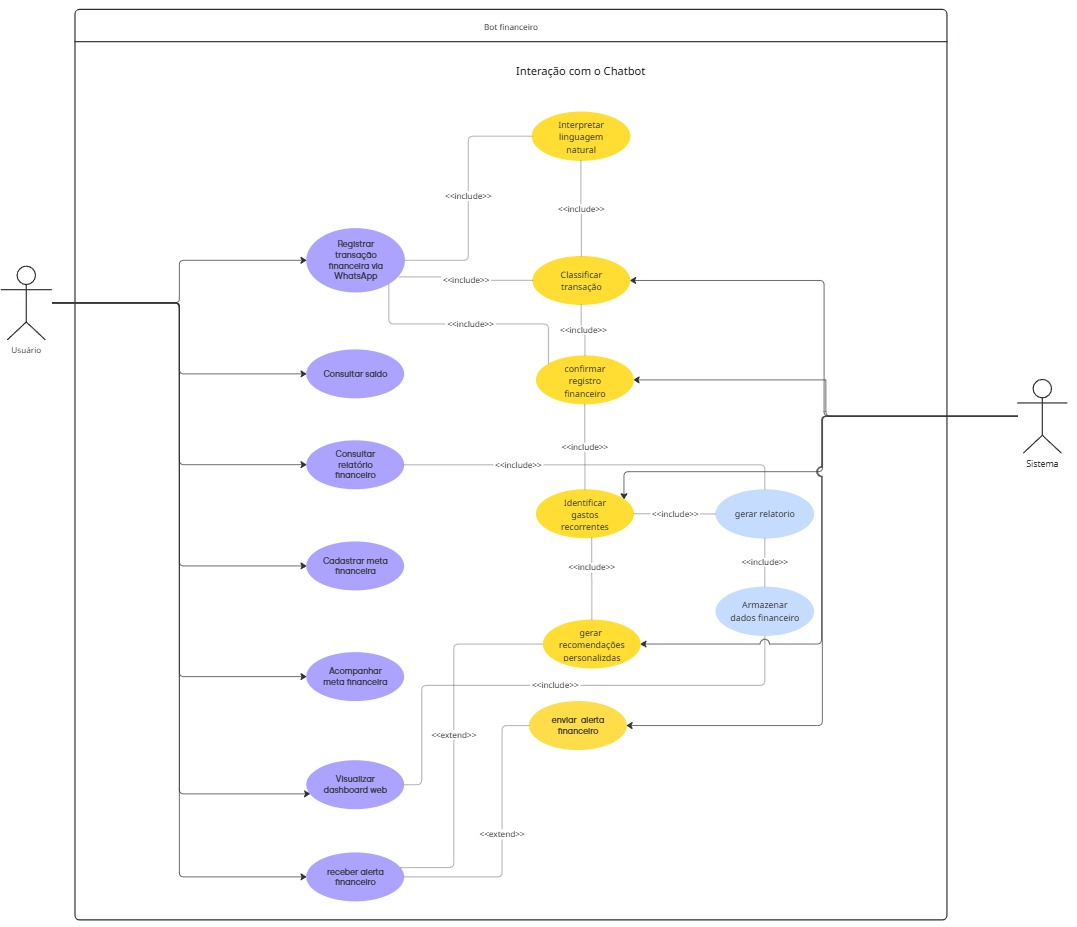
\includegraphics[width=0.8\textwidth,height=0.60\textheight,keepaspectratio]{figs/diagrama-caso-de-uso.png}
    \fonte{Elaborado pelos autores.}
\end{figure}

\subsubsection{Diagrama de Classes}

O diagrama de classes é um dos diagramas mais utilizados da UML, sendo responsável por representar a estrutura estática de um sistema orientado a objetos. Esse tipo de diagrama permite demonstrar as classes existentes no sistema, seus atributos, métodos e os relacionamentos entre elas. Além disso, o diagrama de classes auxilia na visualização da organização do software, contribuindo para a compreensão da arquitetura do sistema e das responsabilidades de cada componente.

No contexto da presente proposta, o diagrama de classes contempla as entidades centrais pelo gerenciamento de usuários, mensagens, transações financeiras, categorias, metas financeiras e notificações. Além disso, o diagrama também apresenta uma classe de serviço responsável pelas funcionalidades de inteligência artificial, incluindo processamento de mensagens, geração de recomendações e emissão de alertas financeiros. Os relacionamentos apresentados demonstram como os componentes do sistema se conectam,

permitindo a integração entre o controle financeiro, a comunicação conversacional e os recursos inteligentes propostos pela aplicação.

\begin{figure}[htbp]
    \centering
    \caption{Diagrama de classes}
    \label{fig:md-12}
    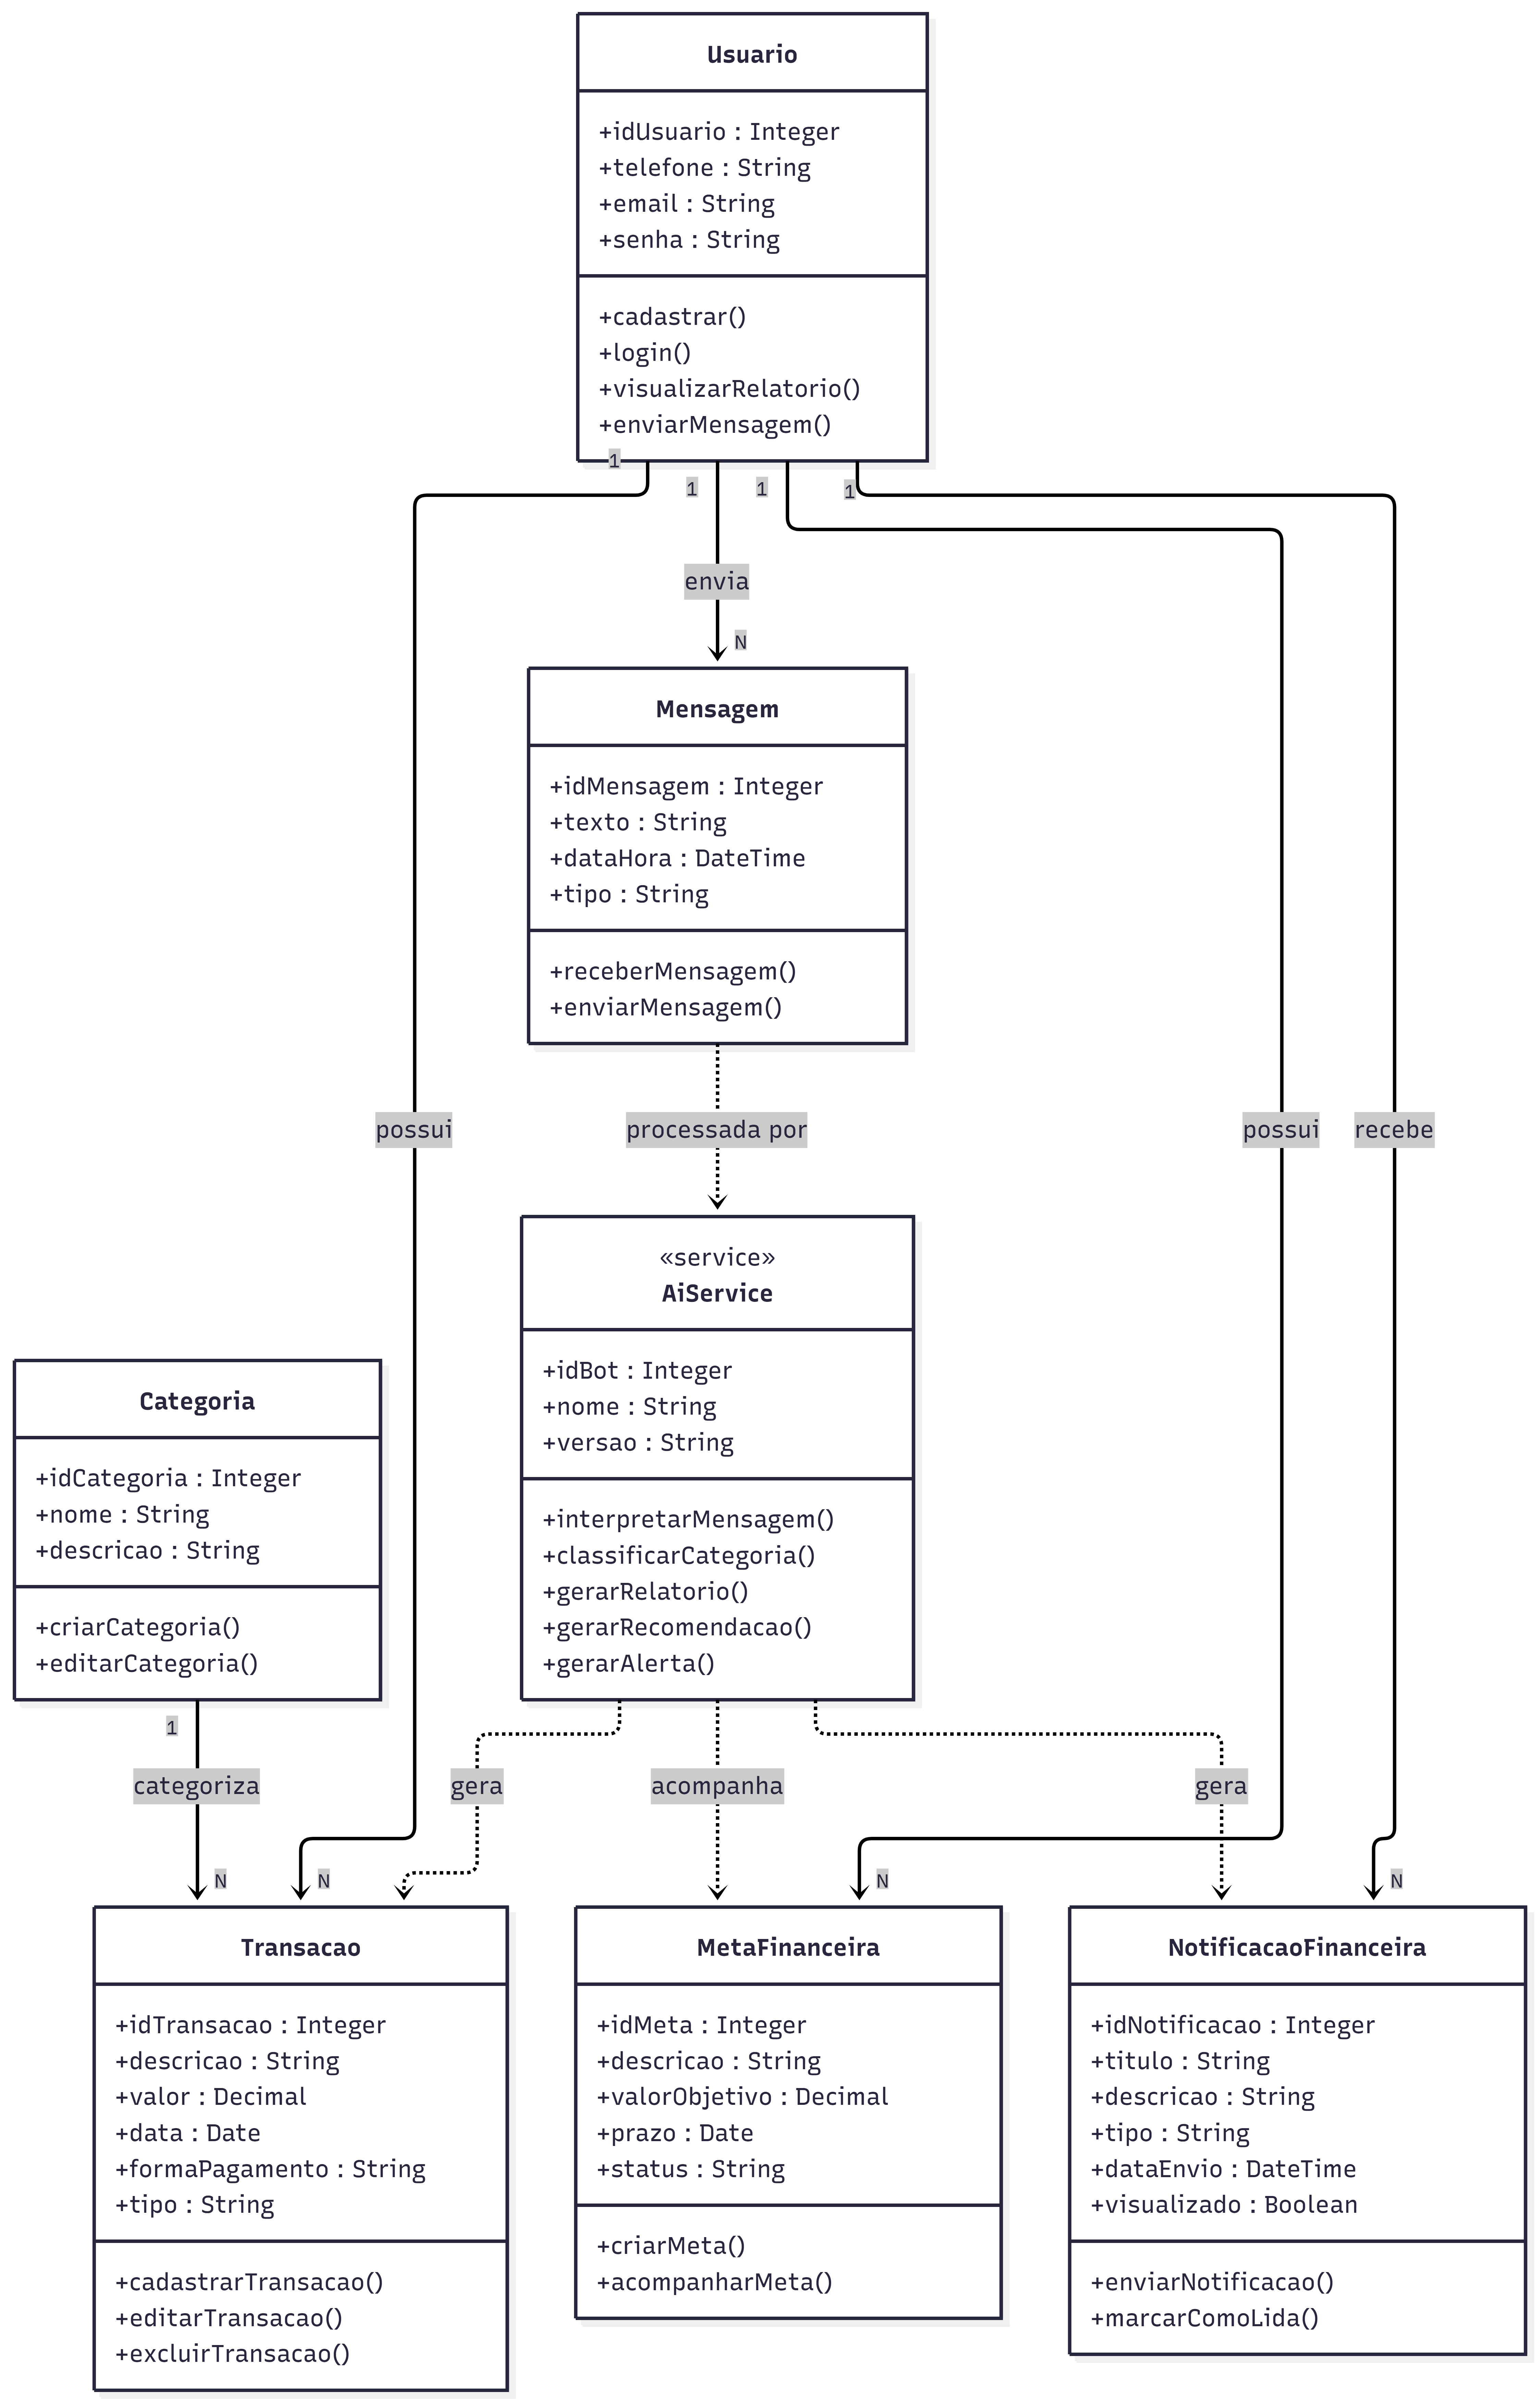
\includegraphics[width=0.8\textwidth,height=0.60\textheight,keepaspectratio]{figs/diagrama-de-classe.png}
    \fonte{Elaborado pelos autores.}
\end{figure}

\subsubsection{Diagrama Entidade-Relacionamento}

O diagrama entidade-relacionamento é uma técnica de modelagem utilizada para representar a estrutura lógica de um banco de dados, permitindo visualizar entidades, atributos e os relacionamentos existentes entre os dados do sistema. Esse tipo de diagrama auxilia na organização e no planejamento do banco de dados, contribuindo para a definição das informações que serão armazenadas e da forma como essas informações se relacionam dentro da aplicação. Além disso, o modelo entidade-relacionamento é amplamente utilizado durante o desenvolvimento de sistemas para facilitar a compreensão da estrutura dos dados e apoiar a implementação do banco de dados.

No contexto da presente proposta, o diagrama entidade-relacionamento representa as principais entidades relacionadas ao gerenciamento financeiro e à comunicação conversacional do sistema. A estrutura contempla entidades responsáveis pelo armazenamento de usuários, conversas, mensagens, transações financeiras, categorias, metas financeiras e notificações. Os relacionamentos apresentados demonstram como essas entidades se conectam dentro do banco de dados, permitindo o gerenciamento das informações financeiras, o armazenamento do histórico de conversas e o envio de notificações ao usuário. Dessa forma, o diagrama evidencia a organização dos dados necessários para o funcionamento da aplicação proposta.

\begin{figure}[htbp]
    \centering
    \caption{Diagrama entidade-relacionamento}
    \label{fig:md-13}
    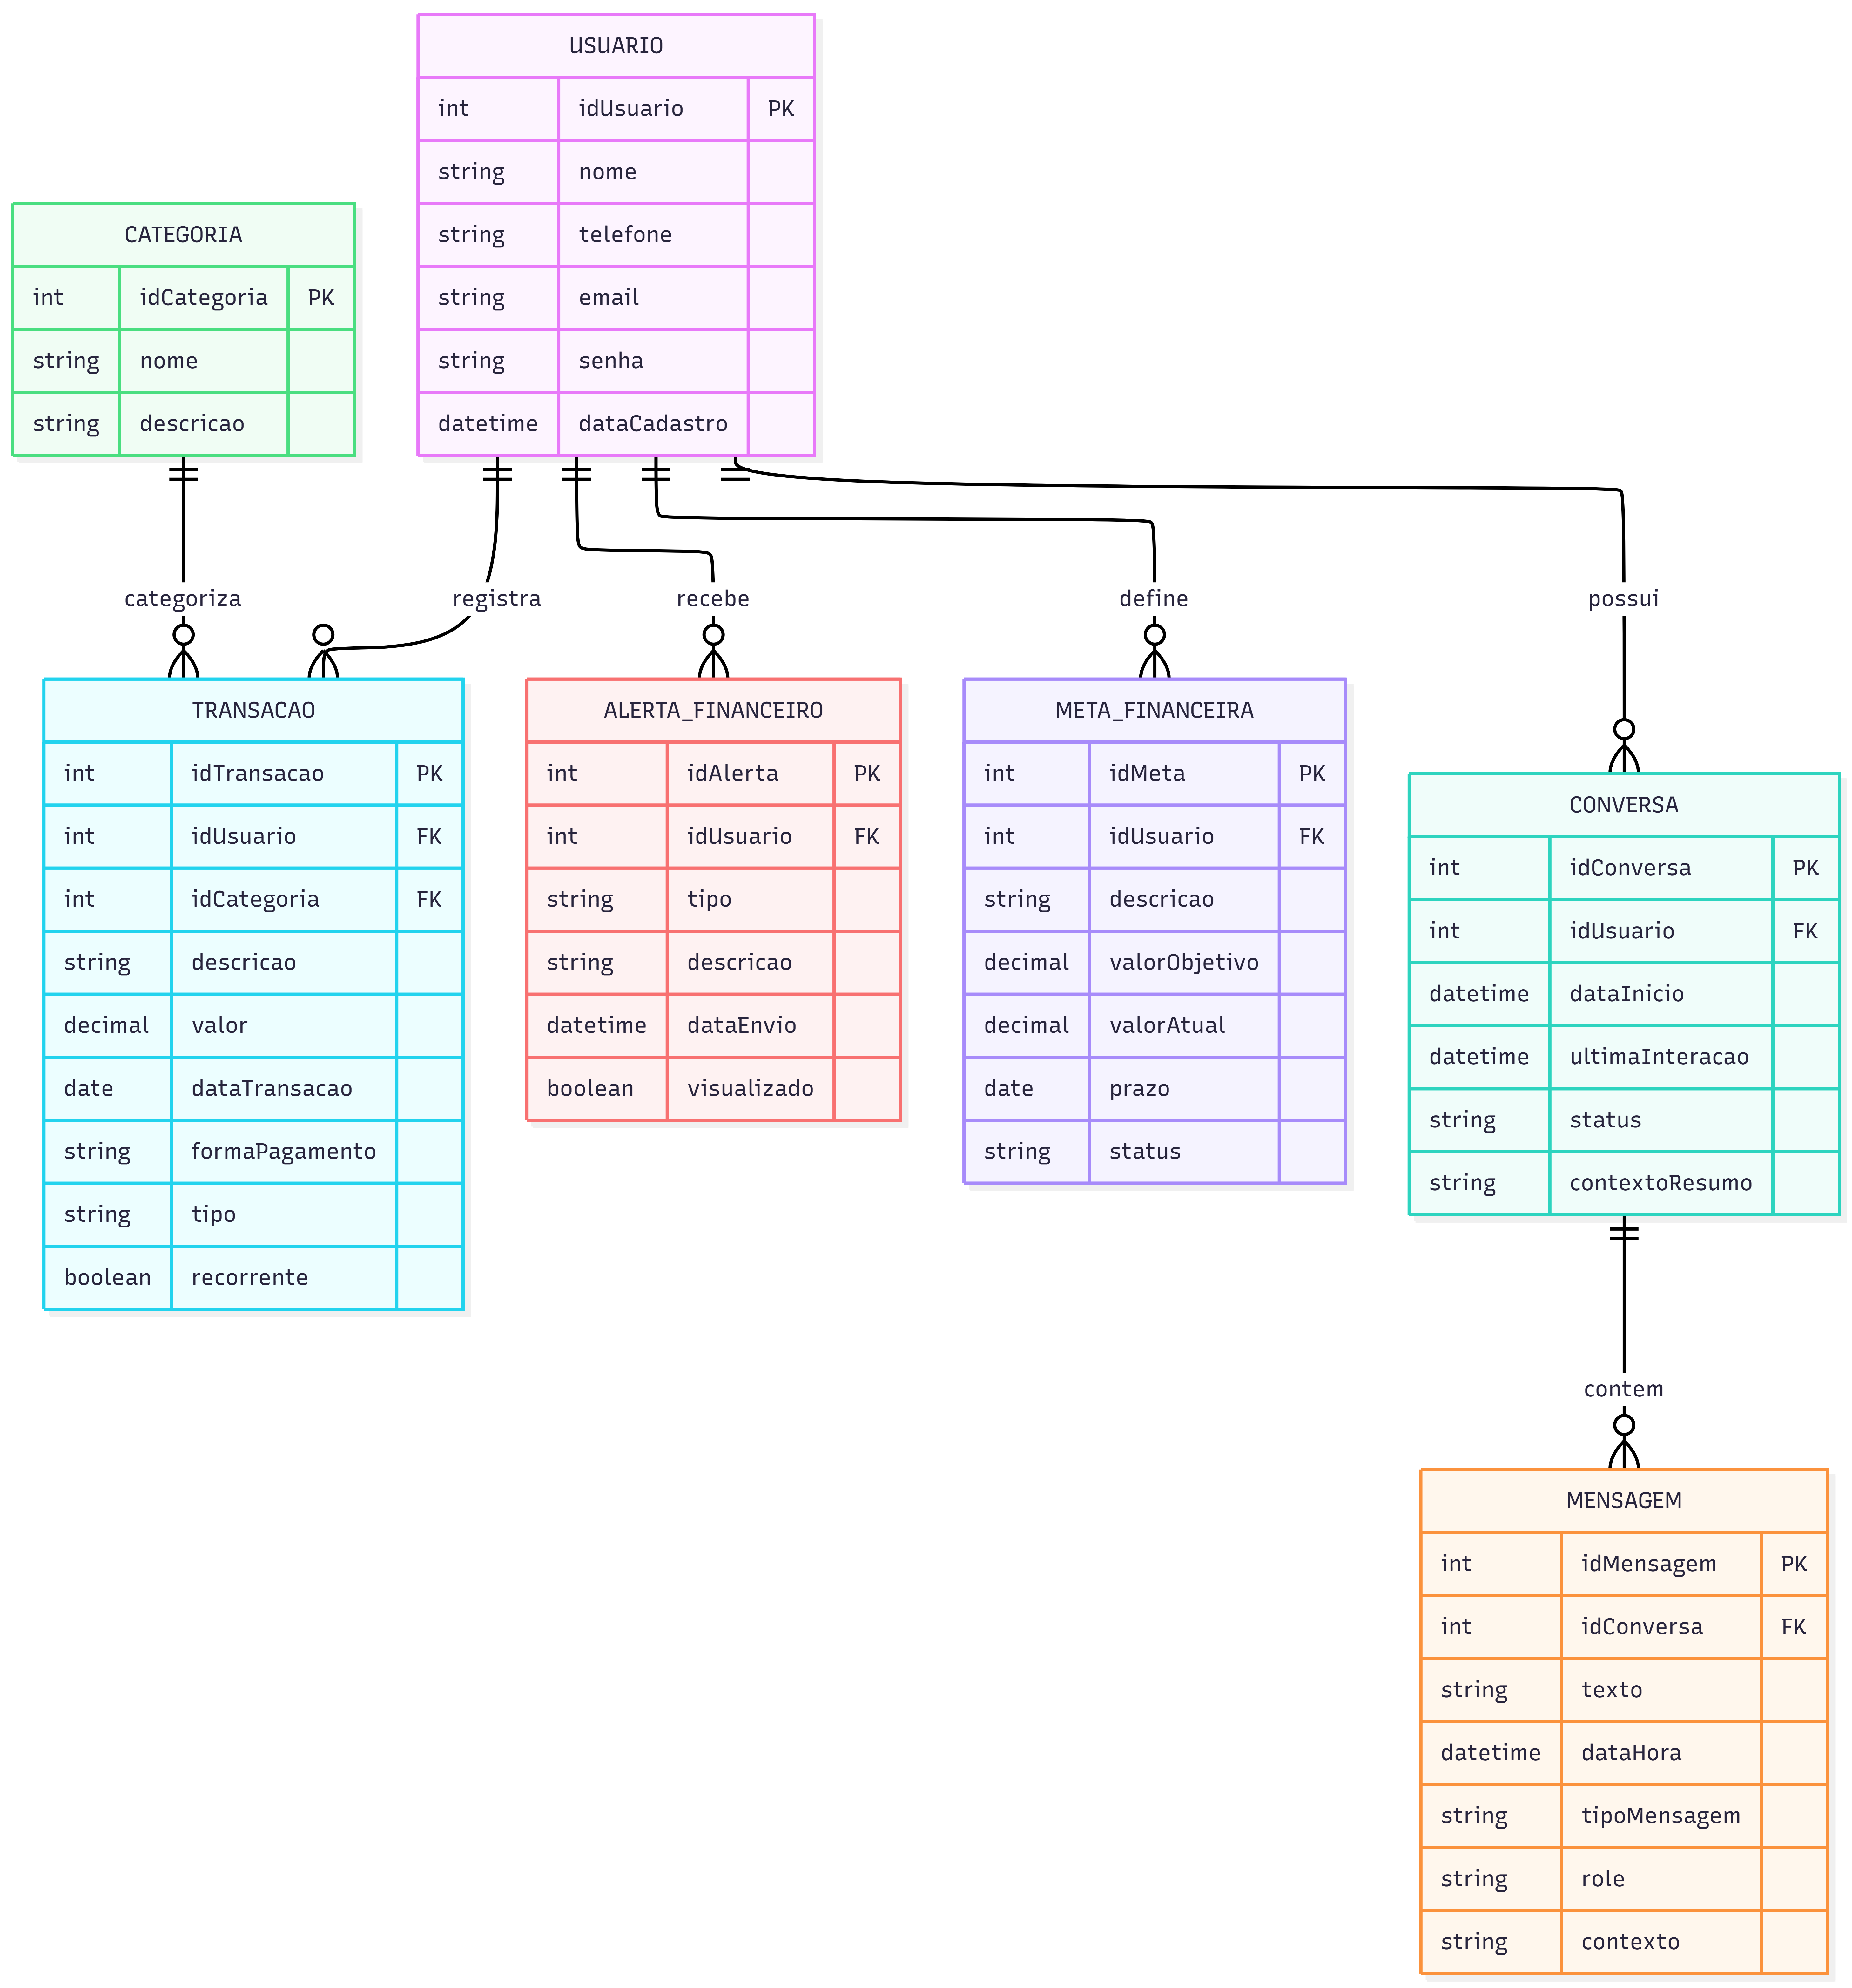
\includegraphics[width=0.8\textwidth,height=0.60\textheight,keepaspectratio]{figs/diagrama-entidade-relacionamento.png}
    \fonte{Elaborado pelos autores.}
\end{figure}

\newlength{\alturaPrint}
\newlength{\larguraPrint}
\newlength{\margemInferiorPrint}
\newlength{\margemSuperiorPrint}
\newcommand{\trechoPrint}[3]{%
    \settoheight{\alturaPrint}{\includegraphics{#1}}%
    \setlength{\margemInferiorPrint}{#2\alturaPrint}%
    \setlength{\margemSuperiorPrint}{#3\alturaPrint}%
    \edef\comandoPrint{\noexpand\includegraphics[width=\larguraPrint,height=0.70\noexpand\textheight,keepaspectratio,trim={0pt \the\margemInferiorPrint\space 0pt \the\margemSuperiorPrint},clip]{#1}}%
    \comandoPrint%
}

\subsection{Interface de Usuário}

A interface da solução reúne a interação conversacional no WhatsApp e a plataforma web de acompanhamento financeiro. As figuras apresentadas nesta subseção mostram as telas do sistema desenvolvido em formato móvel. Algumas incluem o conteúdo completo de uma página com rolagem.

\subsubsection{Fluxo de cadastro e uso do sistema}

O uso da solução proposta pode começar por dois caminhos. No primeiro, o usuário acessa diretamente a versão web do GranaAI, abre a tela de cadastro e preenche as informações solicitadas pelo sistema. Após a conclusão do formulário, a plataforma confirma o cadastro e permite que o usuário siga para o uso da aplicação.

No segundo caminho, o primeiro contato acontece pelo WhatsApp. Caso o usuário envie uma mensagem ao chatbot antes de possuir cadastro, o sistema identifica que aquele número ainda não está vinculado a nenhuma conta. Em seguida, o assistente informa a necessidade de cadastro e envia o link da tela correspondente.

Depois que o cadastro é finalizado, o usuário recebe uma confirmação na versão web e pode retornar à conversa com o chatbot. A partir desse momento, quando ele enviar uma mensagem relacionada a uma movimentação financeira, como uma despesa ou receita, o sistema associa automaticamente o número de telefone à conta cadastrada.

Com essa vinculação, as informações enviadas pelo WhatsApp passam a ser registradas na base de dados do usuário. Assim, uma mensagem como “gastei R\$ 35,00 com lanche” pode ser interpretada pelo chatbot, classificada como despesa e armazenada na categoria correspondente.

Para consultar essas informações na versão web, o usuário acessa a tela de login e informa os dados definidos no cadastro. Após a autenticação, ele visualiza suas movimentações, gráficos, metas financeiras e relatórios gerados a partir dos registros feitos pelo WhatsApp.

\begin{figure}[H]
    \centering
    \caption{Diagrama de sequência de cadastro e registro financeiro}
    \label{fig:md-14}
    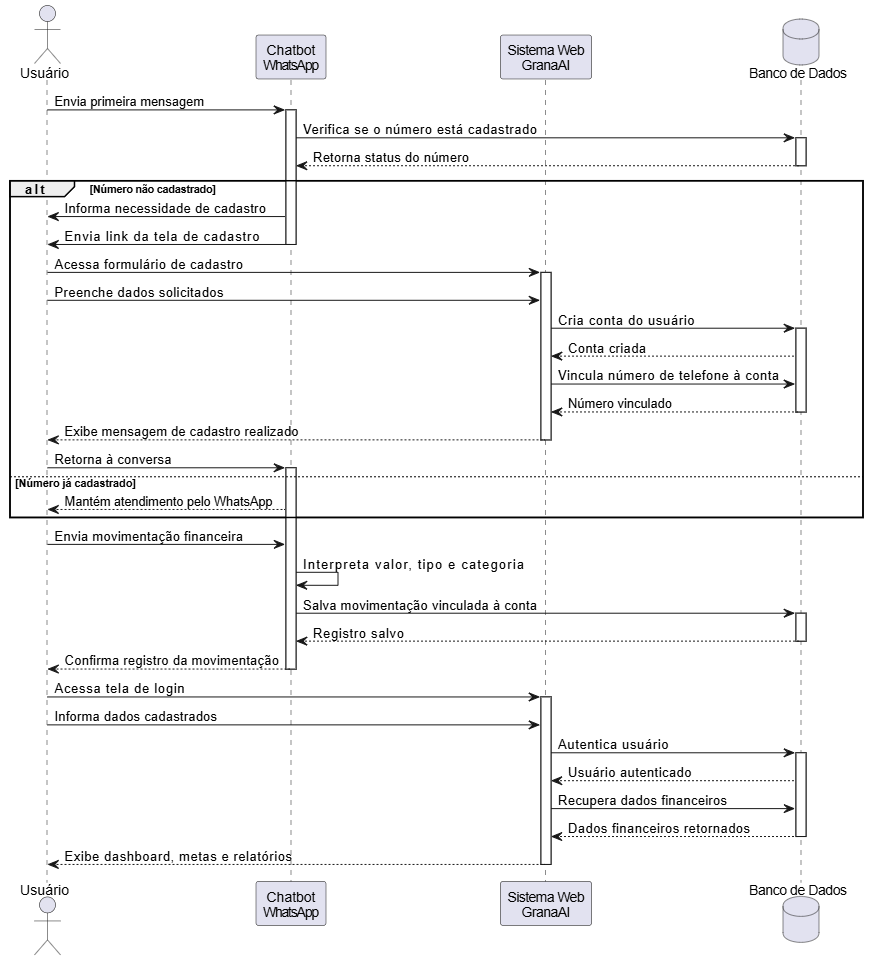
\includegraphics[width=0.8\textwidth,height=0.60\textheight,keepaspectratio]{figs/diagrama-sequencia.png}
    \fonte{Elaborado pelos autores.}
\end{figure}

As telas de cadastro e acesso são apresentadas na Figura~\ref{fig:prints-acesso}. À esquerda, o formulário de criação de conta reúne nome, telefone, e-mail opcional, senha, confirmação de senha e renda mensal. À direita, o formulário de entrada solicita telefone e senha e oferece acesso ao cadastro para quem ainda não possui conta. A comparação mostra a separação entre o preenchimento inicial dos dados e a identificação necessária para acessar a plataforma.

\begin{figure}[H]
    \centering
    \setlength{\larguraPrint}{0.44\textwidth}
    \caption{Telas de cadastro e acesso à plataforma, respectivamente}
    \label{fig:prints-acesso}
    \begin{minipage}[t]{0.48\textwidth}
        \vspace{0pt}\centering
        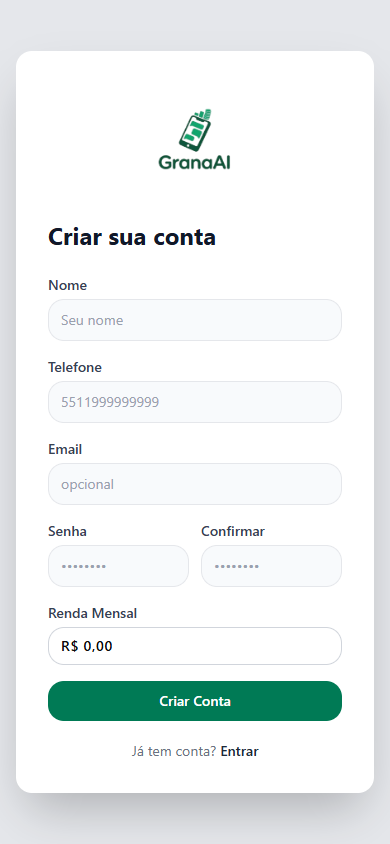
\includegraphics[width=\larguraPrint,height=0.70\textheight,keepaspectratio]{figs/screenshots/cadastro-mobile.png}
    \end{minipage}
    \hfill
    \begin{minipage}[t]{0.48\textwidth}
        \vspace{0pt}\centering
        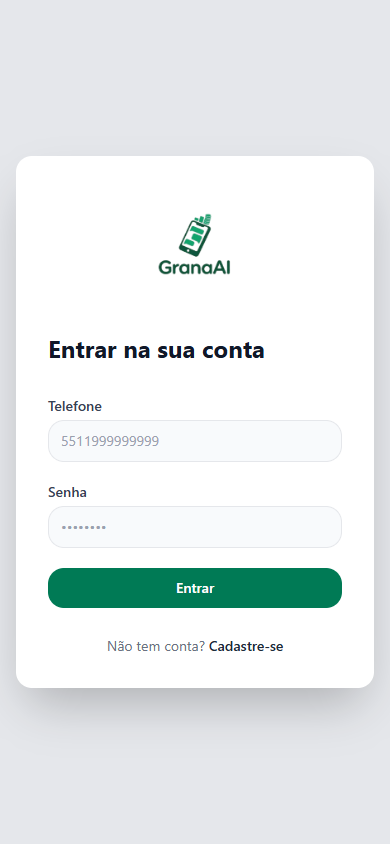
\includegraphics[width=\larguraPrint,height=0.70\textheight,keepaspectratio]{figs/screenshots/login-mobile.png}
    \end{minipage}
    \fonte{Elaboração dos autores a partir da interface do GranaAI.}
\end{figure}

\subsubsection{Interface Conversacional (WhatsApp)}

A interação conversacional foi desenvolvida para receber informações financeiras pelo WhatsApp e encaminhá-las aos serviços da aplicação. As figuras desta subseção apresentam o encaminhamento para cadastro, o registro de uma despesa e as consultas de categorias, metas e assinaturas. Esses fluxos permitem acompanhar a comunicação entre as mensagens enviadas pelo usuário e as respostas do assistente.

A Figura~\ref{fig:wa-cadastro} mostra o primeiro contato de um usuário sem conta vinculada ao número utilizado na conversa. Após a saudação, o assistente informa a necessidade de cadastro e apresenta o endereço da página de criação de conta. O link relaciona o telefone da conversa ao formulário, permitindo que o usuário prossiga na interface web antes de utilizar as operações financeiras. A mensagem final orienta o retorno ao WhatsApp depois dessa etapa.

\begin{figure}[H]
    \centering
    \setlength{\larguraPrint}{0.55\textwidth}
    \caption{Encaminhamento para cadastro a partir do WhatsApp}
    \label{fig:wa-cadastro}
    \trechoPrint{figs/screenshots/whatsapp-cadastro.png}{0.531250}{0.000000}
    \fonte{Elaboração dos autores a partir da interface do GranaAI no WhatsApp.}
\end{figure}

A sequência apresentada na Figura~\ref{fig:md-15} mostra o registro de uma despesa. O usuário envia a mensagem \textit{Pizza 45 reais}, e o assistente organiza o valor, a categoria Alimentação e a descrição Pizza em um resumo. Antes da gravação, a resposta solicita que o usuário digite sim para confirmar ou não para cancelar. Após a resposta afirmativa, o assistente informa a conclusão do registro e repete os dados da movimentação, permitindo conferir o resultado da operação na própria conversa.

\begin{figure}[H]
    \centering
    \setlength{\larguraPrint}{0.55\textwidth}
    \caption{Registro e confirmação de despesa pelo WhatsApp}
    \label{fig:md-15}
    \trechoPrint{figs/screenshots/whatsapp-despesa.jpeg}{0.122500}{0.000000}
    \fonte{Elaboração dos autores a partir da interface do GranaAI no WhatsApp.}
\end{figure}

As consultas de categorias e metas são apresentadas na Figura~\ref{fig:wa-categorias-metas}. À esquerda, a mensagem \textit{Minhas categorias} retorna a relação de categorias com o valor utilizado, o limite e o percentual correspondente. Essa apresentação reúne o acompanhamento do orçamento na conversa, sem exigir a abertura da página de categorias. À direita, a solicitação \textit{Minhas metas} apresenta os objetivos cadastrados, os valores acumulados, os valores-alvo e os percentuais de progresso. Os dois fluxos permitem consultar informações organizadas pelo sistema por meio de mensagens curtas.

\begin{figure}[H]
    \centering
    \setlength{\larguraPrint}{0.44\textwidth}
    \caption{Consulta de categorias e metas pelo WhatsApp}
    \label{fig:wa-categorias-metas}
    \begin{minipage}[t]{0.48\textwidth}
        \vspace{0pt}\centering
        \trechoPrint{figs/screenshots/whatsapp-categorias.jpeg}{0.125000}{0.000000}
    \end{minipage}
    \hfill
    \begin{minipage}[t]{0.48\textwidth}
        \vspace{0pt}\centering
        \trechoPrint{figs/screenshots/whatsapp-metas.jpeg}{0.500000}{0.000000}
    \end{minipage}
    \fonte{Elaboração dos autores a partir da interface do GranaAI no WhatsApp.}
\end{figure}

A Figura~\ref{fig:wa-assinaturas} apresenta a consulta de assinaturas. Ao receber a mensagem \textit{Minhas assinaturas}, o assistente retorna os serviços acompanhados, seus valores mensais e os dias de cobrança. A resposta também destaca as assinaturas ainda não cobradas no mês, reunindo informações sobre os compromissos recorrentes em uma única mensagem. Essa consulta complementa a página de assinaturas da interface web e permite acompanhar as cobranças diretamente pelo WhatsApp.

\begin{figure}[H]
    \centering
    \setlength{\larguraPrint}{0.55\textwidth}
    \caption{Consulta de assinaturas e cobranças pelo WhatsApp}
    \label{fig:wa-assinaturas}
    \trechoPrint{figs/screenshots/whatsapp-assinaturas.jpeg}{0.493750}{0.000000}
    \fonte{Elaboração dos autores a partir da interface do GranaAI no WhatsApp.}
\end{figure}

\subsubsection{Dashboard Web}

A plataforma web organiza a consulta e o gerenciamento das informações financeiras em páginas específicas. O menu apresentado na Figura~\ref{fig:prints-menu} permite acessar início, transações, categorias, metas, assinaturas e relatórios. O destaque sobre Início identifica a página selecionada, enquanto o conteúdo ao fundo permanece escurecido durante a abertura do menu.

\begin{figure}[H]
    \centering
    \setlength{\larguraPrint}{0.44\textwidth}
    \caption{Menu de navegação da interface móvel}
    \label{fig:prints-menu}
    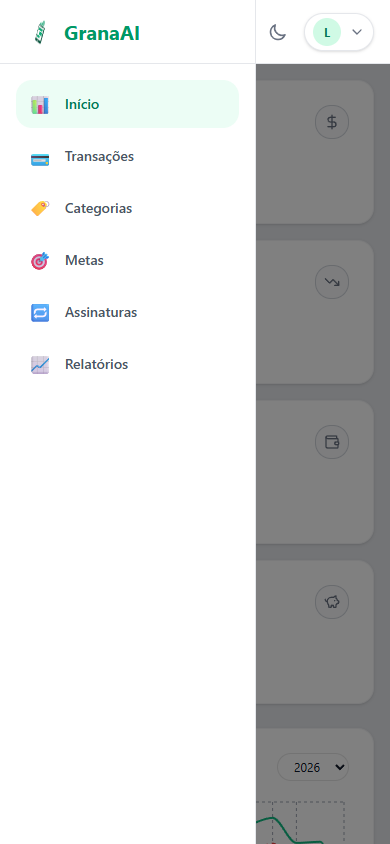
\includegraphics[width=\larguraPrint,height=0.70\textheight,keepaspectratio]{figs/screenshots/menu-inicio-mobile.png}
    \fonte{Elaboração dos autores a partir da interface do GranaAI.}
\end{figure}

\paragraph{Visão geral do painel}

\begin{samepage}
A Figura~\ref{fig:md-16} apresenta o painel inicial. À esquerda, estão os cartões de receitas, despesas, valor líquido e disponibilidade livre de metas. No backend, receitas e despesas do mês são calculadas separadamente do saldo acumulado, e a disponibilidade considera a reserva associada às metas.
\end{samepage}

À direita, são apresentados a análise do fluxo de caixa, a distribuição de despesas e o comparativo mensal. No gráfico de fluxo de caixa, o eixo horizontal representa os meses e o eixo vertical os valores monetários, com séries distintas para receitas, despesas e resultado líquido.

\begin{figure}[H]
    \centering
    \setlength{\larguraPrint}{0.44\textwidth}
    \caption{Indicadores e gráficos do painel inicial}
    \label{fig:md-16}
    \begin{minipage}[t]{0.48\textwidth}
        \vspace{0pt}\centering
        \trechoPrint{figs/screenshots/painel-mobile.png}{0.596865}{0.000000}
    \end{minipage}
    \hfill
    \begin{minipage}[t]{0.48\textwidth}
        \vspace{0pt}\centering
        \trechoPrint{figs/screenshots/painel-mobile.png}{0.000000}{0.403135}
    \end{minipage}
    \fonte{Elaboração dos autores a partir da interface do GranaAI.}
\end{figure}

\paragraph{Transações e registro manual}

A Figura~\ref{fig:prints-transacoes} mostra a listagem de transações. A tela oferece exportação CSV, criação de transação e filtros por mês, ano, categoria e tipo, além dos comandos para aplicar ou limpar a seleção. Na parte da listagem, são apresentados descrição, data, categoria e valor das despesas, com ações de edição e exclusão. O controle de paginação permite escolher a quantidade de itens por página e percorrer os registros. Esses elementos permitem filtrar os dados e consultar as movimentações registradas.

\begin{figure}[H]
    \centering
    \setlength{\larguraPrint}{0.44\textwidth}
    \caption{Listagem de transações}
    \label{fig:prints-transacoes}
    \trechoPrint{figs/screenshots/transacoes-mobile.png}{0.707034}{0.000000}
    \fonte{Elaboração dos autores a partir da interface do GranaAI.}
\end{figure}

O formulário de lançamento manual é apresentado na Figura~\ref{fig:prints-nova-transacao}. Nele, o usuário informa o tipo da movimentação, o valor, a descrição, a categoria e a data. Os campos marcados com asterisco indicam os preenchimentos exigidos pela interface. Sobre a categoria, existe a possibilidade de criação de uma categoria nova ao salvar, e os botões finais permitem cancelar ou encaminhar o registro.

\begin{figure}[H]
    \centering
    \setlength{\larguraPrint}{0.44\textwidth}
    \caption{Formulário de nova transação}
    \label{fig:prints-nova-transacao}
    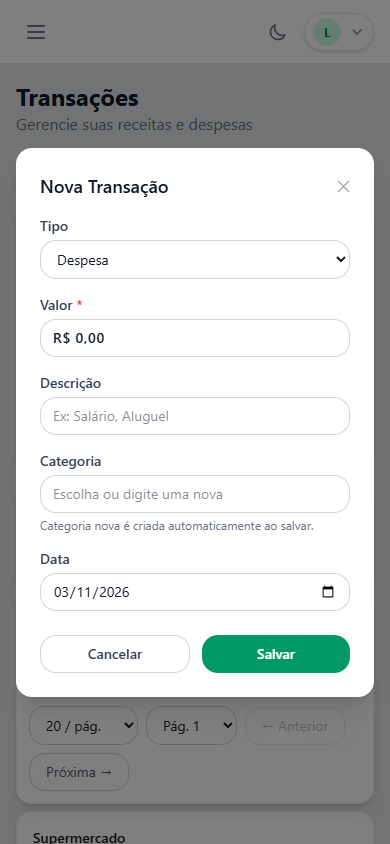
\includegraphics[width=\larguraPrint,height=0.70\textheight,keepaspectratio]{figs/screenshots/nova-transacao-mobile.png}
    \fonte{Elaboração dos autores a partir da interface do GranaAI.}
\end{figure}

\paragraph{Categorias e limites}

A Figura~\ref{fig:md-17} apresenta a página de categorias. A parte superior contém seleção de período, pesquisa e filtros para categorias com ou sem gastos. Cada cartão identifica a categoria, o limite, o valor gasto e o valor restante, acompanhado de uma barra de utilização e dos comandos de edição e exclusão. 

\begin{figure}[H]
    \centering
    \setlength{\larguraPrint}{0.44\textwidth}
    \caption{Consulta de categorias e limites mensais}
    \label{fig:md-17}
    \begin{minipage}[t]{0.48\textwidth}
        \vspace{0pt}\centering
        \trechoPrint{figs/screenshots/categorias-mobile.png}{0.450711}{0.000000}
    \end{minipage}
    \hfill
    \begin{minipage}[t]{0.48\textwidth}
        \vspace{0pt}\centering
        \trechoPrint{figs/screenshots/categorias-mobile.png}{0.000000}{0.549289}
    \end{minipage}
    \fonte{Elaboração dos autores a partir da interface do GranaAI.}
\end{figure}

O cadastro de categoria, apresentado na Figura~\ref{fig:prints-nova-categoria}, reúne nome, limite mensal, ícone e cor. Os dois últimos elementos organizam a identificação visual dos cartões, enquanto o limite fornece o valor de referência para acompanhar o orçamento daquela categoria. O formulário também oferece cancelamento e gravação.

\begin{figure}[H]
    \centering
    \setlength{\larguraPrint}{0.44\textwidth}
    \caption{Formulário de cadastro de categoria}
    \label{fig:prints-nova-categoria}
    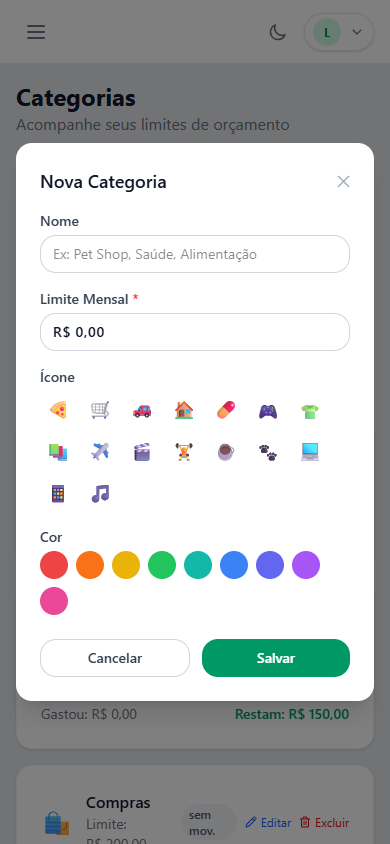
\includegraphics[width=\larguraPrint,height=0.70\textheight,keepaspectratio]{figs/screenshots/nova-categoria-mobile.png}
    \fonte{Elaboração dos autores a partir da interface do GranaAI.}
\end{figure}

\paragraph{Metas financeiras}

As telas da Figura~\ref{fig:md-18} apresentam a consulta e a criação de metas. Na listagem, cada cartão mostra o título do objetivo, os valores atual e desejado, a barra de progresso e as opções de edição e exclusão. A pesquisa e os filtros permitem selecionar metas ativas ou concluídas. Ao lado, o formulário de nova meta solicita título e valor-alvo, com comandos para salvar ou cancelar a inclusão.

\begin{figure}[H]
    \centering
    \setlength{\larguraPrint}{0.44\textwidth}
    \caption{Consulta de metas financeiras e formulário de nova meta}
    \label{fig:md-18}
    \begin{minipage}[t]{0.48\textwidth}
        \vspace{0pt}\centering
        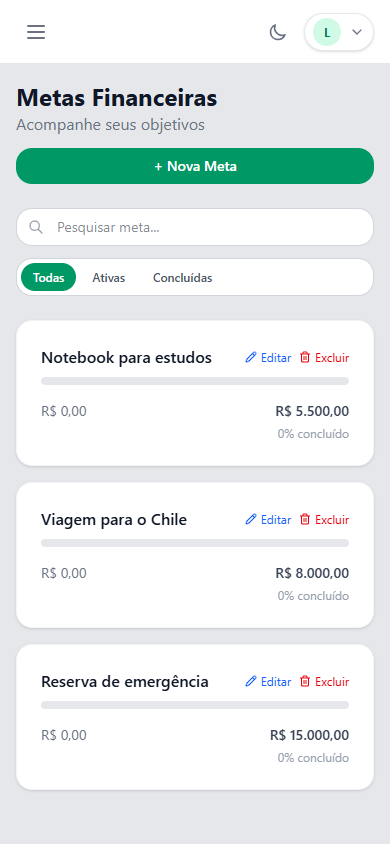
\includegraphics[width=\larguraPrint,height=0.70\textheight,keepaspectratio]{figs/screenshots/metas-mobile.png}
    \end{minipage}
    \hfill
    \begin{minipage}[t]{0.48\textwidth}
        \vspace{0pt}\centering
        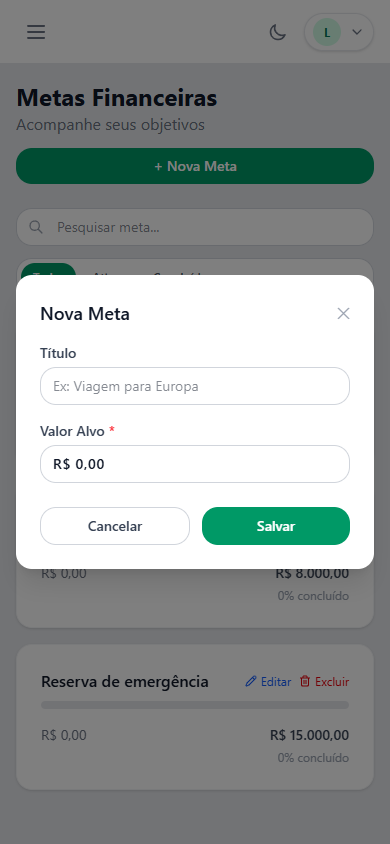
\includegraphics[width=\larguraPrint,height=0.70\textheight,keepaspectratio]{figs/screenshots/nova-meta-mobile.png}
    \end{minipage}
    \fonte{Elaboração dos autores a partir da interface do GranaAI.}
\end{figure}

\paragraph{Assinaturas e cobranças recorrentes}

A Figura~\ref{fig:prints-assinaturas} apresenta a página de assinaturas. A interface distingue cobranças previstas no mês, padrões detectados automaticamente e assinaturas que já estão sendo acompanhadas. Na área de detecção, os cartões apresentam descrição, valor, categoria, quantidade de meses e dia associado à cobrança, com a ação Acompanhar. Na área de assinaturas do usuário, aparecem classificação como necessária ou dispensável e comandos de edição e exclusão.

\begin{figure}[H]
    \centering
    \setlength{\larguraPrint}{0.44\textwidth}
    \caption{Acompanhamento de assinaturas e cobranças}
    \label{fig:prints-assinaturas}
    \begin{minipage}[t]{0.48\textwidth}
        \vspace{0pt}\centering
        \trechoPrint{figs/screenshots/assinaturas-mobile.png}{0.475628}{0.000000}
    \end{minipage}
    \hfill
    \begin{minipage}[t]{0.48\textwidth}
        \vspace{0pt}\centering
        \trechoPrint{figs/screenshots/assinaturas-mobile.png}{0.000000}{0.524372}
    \end{minipage}
    \fonte{Elaboração dos autores a partir da interface do GranaAI.}
\end{figure}

A Figura~\ref{fig:prints-nova-assinatura} apresenta o formulário de inclusão manual de uma assinatura. Os campos visíveis permitem indicar nome, categoria, valor mensal e dia da cobrança. Essa entrada complementa a identificação automática ao oferecer uma forma de cadastrar um compromisso conhecido pelo usuário. Os botões Cancelar e Salvar encerram a operação sem inclusão ou encaminham os dados para gravação, respectivamente.

\begin{figure}[H]
    \centering
    \setlength{\larguraPrint}{0.44\textwidth}
    \caption{Formulário de nova assinatura}
    \label{fig:prints-nova-assinatura}
    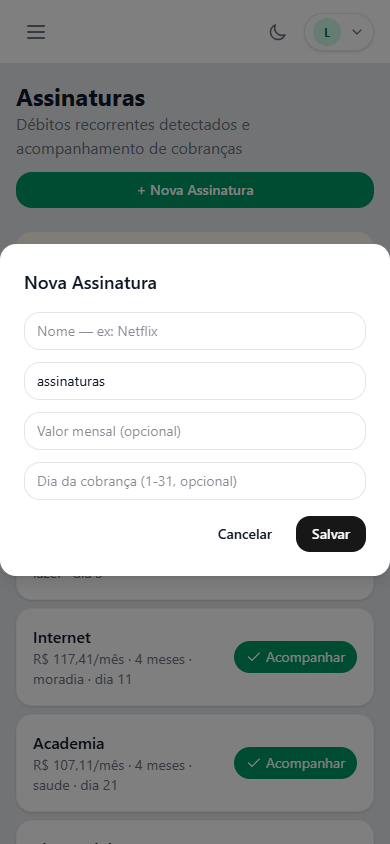
\includegraphics[width=\larguraPrint,height=0.70\textheight,keepaspectratio]{figs/screenshots/nova-assinatura-mobile.png}
    \fonte{Elaboração dos autores a partir da interface do GranaAI.}
\end{figure}

\paragraph{Relatórios, tendências e projeções}

A Figura~\ref{fig:md-19} apresenta o resumo financeiro e a análise de tendência. À esquerda, estão receitas, despesas e saldo do período indicado, além das mensagens na área de \textit{insights}.

À direita, estão o gráfico de tendência e a tabela que o acompanha. O eixo horizontal organiza os períodos e o vertical representa valores monetários, com séries diferenciadas para receitas e despesas. A tabela discrimina os mesmos tipos de informação por mês, permitindo consultar os valores numéricos além da representação gráfica.

\begin{figure}[H]
    \centering
    \setlength{\larguraPrint}{0.44\textwidth}
    \caption{Resumo financeiro e análise de tendência}
    \label{fig:md-19}
    \begin{minipage}[t]{0.48\textwidth}
        \vspace{0pt}\centering
        \trechoPrint{figs/screenshots/relatorios-mobile.png}{0.695200}{0.000000}
    \end{minipage}
    \hfill
    \begin{minipage}[t]{0.48\textwidth}
        \vspace{0pt}\centering
        \trechoPrint{figs/screenshots/relatorios-mobile.png}{0.438400}{0.304800}
    \end{minipage}
    \fonte{Elaboração dos autores a partir da interface do GranaAI.}
\end{figure}

A projeção exibida na Figura~\ref{fig:prints-projecao} apresenta um gráfico de saldo acumulado e uma tabela com receitas, despesas e saldo projetados para os meses seguintes. Para estimar os próximos meses, o sistema calcula a média das receitas e das despesas já registradas. A diferença entre essas médias é somada ao saldo a cada mês da projeção. Abaixo do gráfico, são informados os valores usados nessa estimativa.

\begin{figure}[H]
    \centering
    \setlength{\larguraPrint}{0.44\textwidth}
    \caption{Projeção financeira para os períodos seguintes}
    \label{fig:prints-projecao}
    \trechoPrint{figs/screenshots/relatorios-mobile.png}{0.129200}{0.561600}
    \fonte{Elaboração dos autores a partir da interface do GranaAI.}
\end{figure}

\paragraph{Perfil e preferências}

A Figura~\ref{fig:prints-perfil} apresenta os campos de telefone, nome, e-mail, renda mensal e personalidade do assistente, além do comando para salvar as preferências. O seletor de personalidade indica a possibilidade de configurar o estilo de comunicação, enquanto os demais campos organizam informações da conta. Para a inclusão na monografia, os valores dos campos pessoais foram ocultados por tarjas aplicadas à cópia da imagem. Os rótulos e os controles foram preservados para permitir a compreensão da tela.

\begin{figure}[H]
    \centering
    \setlength{\larguraPrint}{0.44\textwidth}
    \caption{Tela de perfil com os campos pessoais anonimizados}
    \label{fig:prints-perfil}
    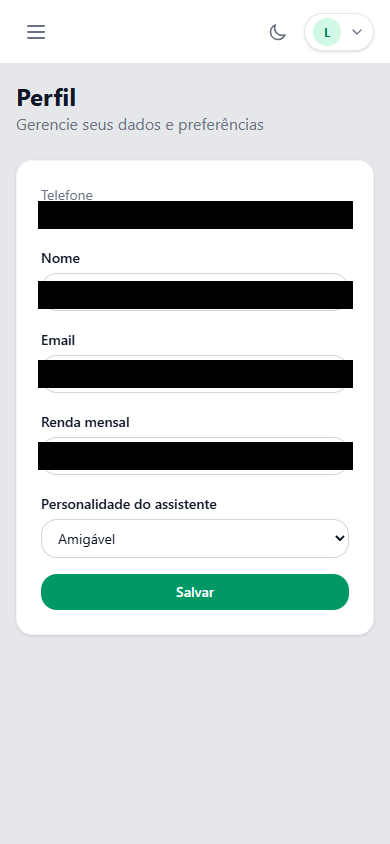
\includegraphics[width=\larguraPrint,height=0.70\textheight,keepaspectratio]{figs/screenshots/perfil-mobile.png}
    \fonte{Elaboração dos autores a partir da interface do GranaAI.}
\end{figure}
